\documentclass[hyperref={pdfpagelabels=false}]{beamer}
\usepackage{lmodern}
\usetheme{Frankfurt}
\usepackage{natbib}
\usepackage{amsmath}
\usepackage{multirow}
\usepackage{graphicx}
\usepackage{listings}
\usepackage{caption}
\usepackage{subcaption}
\usepackage{diagbox}
\usepackage{colortbl}
\usepackage{graphicx}
\usepackage{tikz}
\usetikzlibrary{arrows,shapes,snakes,automata,backgrounds,petri}
\usepackage{geometry}
\lstset{basicstyle=\ttfamily, escapeinside={\%*}{*)}}

\title{The role of synergy in the memory and resilience of random discrete gene regulatory networks}
\author{Dylan Goldsborough}
\date{12\textsuperscript{th} of March 2018}

% Citations
\bibliographystyle{plain}

\begin{document}
\begin{frame}
\titlepage
\end{frame} 

%% Structure
\begin{frame}
\frametitle{Table of contents}
\tableofcontents
\end{frame} 

%% LOOP DOOR MIJN THESIS HEEN EN VIND DE JUISTE ZINNEN MET REFERENCES

%%% Introduction
\section{Introduction} 
\setcounter{subsection}{1}

% STORY: I have always found this fascinating, how a complicated system can both attribuate to stability and chaos
% I should tell why absence and excess both change this
%
\begin{frame}
\frametitle{Introduction}
\begin{itemize}
\item Many natural systems are complex
\begin{itemize}
\item Consist of many units
\item Local interactions between units
\item Emergent properties at a larger scale
\end{itemize}
\item Both absence and excess of complexity can reduce system resilience \cite{kondoh2003foraging, macarthur1955fluctuations} \dots{}
\begin{itemize}
\item No complete consensus on the underlying mechanism
\item Less importance of a single interaction?
\item Vulnerability of very complex systems to cascades?
\end{itemize}
\item What is the relationship between complexity and resilience in biological complex systems? 
\end{itemize}
\end{frame}

% STORY: Rick did research into synergy, found that it helps resilience
% Natural systems can only remain in existence if they can cope with the perturbations
\begin{frame}
\frametitle{Introduction}
\begin{itemize}
\item Suggested that synergy increases the resilience of a system against perturbations \cite{quax2017quantifying}
\item Natural systems require two things to operate \dots{}
\begin{itemize}
\item Resilience against single-variable perturbations
\item Retention of information over time ("memory")
\end{itemize}
\item Extreme memory brings low resilience
\item To function well, systems should optimize a combination of memory and resilience\\
\item \textbf{What if synergy plays a role in optimizing this balance?}
\end{itemize}
\end{frame}

\begin{frame}
\frametitle{Introduction}
\begin{itemize}
\item Focus so far on dyadic interactions of variables \cite{ideker2001integrated, lu2004gene, tononi1999measures}
\begin{itemize}
\item Mutual information between random variables
\item Correlations between gene expression
\end{itemize}
\item Synergy is a polyadic interaction
\item Allows us to investigate properties that emerge at the polyadic level\\
\item \textbf{Maybe this is a piece of the puzzle of the relationship between complexity, resilience and memory?}
\end{itemize}
\end{frame}

\begin{frame}
\frametitle{Introduction: Partial information decomposition}
Let us consider a system with random variables $X$ and $Y$ predicting $Z$ \dots{}
\begin{itemize}
\item Unique information, predicts $Z$ contained only in $X$ or $Y$
\item Redundant information, predicts $Z$ contained in both $X$ and $Y$
\item Synergistic information, predicts $Z$ contained in neither $X$ and $Y$, but derived from a combination of the two
\end{itemize}
\end{frame}


\begin{frame}
\frametitle{Introduction: partial information decomposition}
%% PICTURE %%
\def\firstcircle{(0:-0.9cm) circle (2cm)}
\def\secondcircle{(0:0cm) circle (3cm)}
\def\thirdcircle{(0:0.9cm) circle (2cm)}
\begin{figure}[ht]
\begin{center}
\begin{tikzpicture}
    \draw \firstcircle;
    \draw \secondcircle;
    \draw \thirdcircle;
   
    \begin{scope}[fill opacity=0.5]
        \clip \firstcircle;
        \fill[orange] \thirdcircle;
    \end{scope}
   
    \begin{scope}[even odd rule, fill opacity=0.5]
        \clip \thirdcircle (-3,-3) rectangle (3,3);
        \fill[yellow] \firstcircle;
    \end{scope}
   
    \begin{scope}[even odd rule, fill opacity=0.5]
        \clip \firstcircle (-3,-3) rectangle (3,3);
        \fill[red] \thirdcircle;
    \end{scope}
   
    \begin{scope}[even odd rule, fill opacity=0.3]
        \clip \firstcircle (-4,-4) rectangle (4,4);
        \clip \thirdcircle (-4,-4) rectangle (4,4);
        \fill[blue] \secondcircle;
    \end{scope}
   
    \node (x) at (-2,0)  {$\mathrm{I}\left(Z; X \right)$};
    \node (y) at (2,0)   {$\mathrm{I}\left(Z; Y \right)$};
    \node (r) at (0,0)   {$\mathrm{I}_\mathrm{red}\left( Z;X,Y \right)$};
    \node (s) at (0,2.3) {$\mathrm{I}_\mathrm{syn}\left( Z;X,Y \right)$};
    \node (w) at (0,3.2) {$\mathrm{I}\left( Z;X,Y \right)$};
\end{tikzpicture}
\end{center}
\label{venn}
\end{figure}
\end{frame}

% To set the expectations, kind of like the abstract
% Mention that the last two are double, we test it for both but found no difference
\begin{frame}
\frametitle{Research question}
\center{\textbf{Is there a form of synergistic control on memory and resilience in gene regulatory networks?}}\\
\begin{itemize}
\item Comparison of BRM and URM
\item Hypotheses \dots{}
\begin{itemize}
\item There is significantly more synergy in a BRM than in a URM
\item A BRM scores better in memory than a URM
\item A BRM scores better in single-nudge resilience than a URM
\item There is a positive correlation between synergy and resilience
\item There is a positive correlation between synergy and memory
\end{itemize}
\end{itemize}
\end{frame}

\section{Methodology}
\setcounter{subsection}{1}

%TODO continuous was too expensive, mention this
\begin{frame}
\frametitle{A model for GRNs}
\begin{itemize}
\item We model GRN motifs as discrete networks
\begin{itemize}
\item A total of $n$ genes
\item Gene can be in state $m \in \{0, 1, ..., l - 1 \}$
\item Time is discrete and deterministic
\end{itemize}
%\begin{itemize}
%\item Only accurate locally in time, as we omit the rest of the network
%\end{itemize}
\item Joint PMF describes distribution over all system states
\item Initial distribution defined in a correlation matrix
\item Two representations in Python-implementation
\begin{itemize}
\item Graph form
\item Transition table form
\end{itemize}
\end{itemize}
\end{frame}

\begin{frame}
\frametitle{Graph form}
\begin{itemize}
\item Graph form mimics real GRN motifs
\item Nodes and directed edges
\item Genes can have four types of relations
\begin{itemize}
\item Stimulation (+)
\item Inhibition (-)
\item AND-stimulation (mimics co-factor)
\item AND-inhibition (mimics co-factor)
\end{itemize}
\item Non-stimulated genes experience decay over time
\item Self-stimulation is allowed \cite{thomas1995dynamical, zhou2016relative}
\end{itemize}
\end{frame}

\begin{frame}
\frametitle{Graph form}
\begin{figure}
\begin{center}
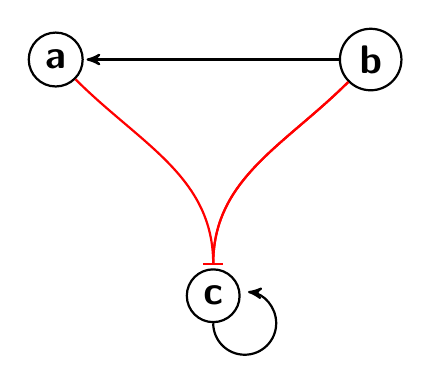
\begin{tikzpicture}[->,>=stealth',auto,node distance=3cm,
  thick,main node/.style={circle,draw,font=\sffamily\Large\bfseries}]

  \node[main node] (1) at (2,0) {c};
  \node[main node] (2) at (0,3) {a};
  \node[main node] (3) at (4,3) {b};

  %\path[every node/.style={font=\sffamily\small}]
  %  (3) edge node [right] {} (2)
  %  (3) edge[bend right=33] node [left] {} (1)
  %  (2) edge[bend left=33] node [right] {} (1);
  \draw[black,thick,->,shorten >=1pt] (3) to [out=180,in=0] (2);
  \draw[red,thick,-|,shorten >=1pt] (3) to [out=225,in=90] (1);
  \draw[red,thick,-|,shorten >=1pt] (3) to [out=225,in=90] (1);
  \draw[red,thick,-|,shorten >=1pt] (2) to [out=-45,in=90] (1);
  \draw[black,thick,->] (1.-90) arc (180:180+264:4mm);
\end{tikzpicture}
\end{center}
\end{figure}
\end{frame}

\begin{frame}
\frametitle{Transition table form}
\begin{itemize}
\item We can convert a graph form to a transition table
\item The transition table defines the state of the system at $t + \delta t$ for each possible system state at $t$
%\item Total of $l^n$ states
\end{itemize}
\begin{table}[ht]
\begin{center}
\begin{tabular}{|c|c|c||c|c|c|}
\hline
$A_t$ & $B_t$ & $C_t$ & $A_{t+\delta t}$ & $B_{t+\delta t}$ & $C_{t+\delta t}$ \\
\hline
\hline
1 & 1 & 1 & 0 & 0 & 0 \\
1 & 1 & 0 & 1 & 0 & 1 \\
1 & 0 & 1 & 1 & 1 & 1 \\
1 & 0 & 0 & 0 & 0 & 0 \\
0 & 1 & 1 & 0 & 0 & 1 \\
0 & 1 & 0 & 1 & 0 & 1 \\
0 & 0 & 1 & 0 & 1 & 0 \\
0 & 0 & 0 & 1 & 1 & 1 \\
\hline
\end{tabular}
\end{center}
\caption{Transition table form for $n=3$ and $l=2$}
\end{table}
\end{frame}

\begin{frame}
\frametitle{Generating BRMs}
\begin{itemize}
\item We sample biological random motifs (BRMs) using the Erdos-Renyi algorithm \cite{margolin2006aracne}
\begin{itemize}
\item We run the algorithm twice; for 1-to-1 edges, and for 2-to-1 edges
\item We allow self-referring edges
\end{itemize}
\item A random eligible function is attached to an edge
\item We then convert to a transition table to perform time evolution
\end{itemize}
\end{frame}

\begin{frame}
\frametitle{Generating URMs}
\begin{itemize}
\item We generate a transition table, skipping the graph form
\item We sample uniform random motifs (URMs) using a randomized design
\item Each expression level in the future state is randomly determined
\item We draw from a uniform distribution between $0$ and $l-1$
\end{itemize}
\begin{table}[ht]
\begin{center}
\begin{tabular}{|c|c||c|c|}
\hline
$A_t$ & $B_t$ & $A_{t+\delta t}$ & $B_{t+\delta t}$ \\
\hline
\hline
1 & 1 & ? & ? \\
1 & 1 & ? & ? \\
1 & 0 & ? & ? \\
1 & 0 & ? & ? \\
\hline
\end{tabular}
\end{center}
\caption{Transition table form for $n=3$ and $l=2$}
\end{table}
\end{frame}

\begin{frame}
\frametitle{Measurement methods}
\begin{itemize}
\item We define the memory as the mutual information between the distribution of states at $t$ and $t + \delta t$
\item We use the mean synergy of a cheap upper- and lower bound
\begin{itemize}
\item Better measures require expensive numerical optimization
\item We use the WMS-synergy and the $\mathrm{I}_\mathrm{max}$-synergy
\end{itemize}
\item Resilience we define using the Hellinger distance
\begin{itemize}
\item We nudge the state distribution at time $t$
\item We compare the state distributions at time $t + \delta t$
\end{itemize}
\item We normalize the memory and synergy
%\item Expression: $\mathrm{I}\left(\mathbf{X}_t ; \mathbf{X}_{t + \Delta t}\right)$
%\item We normalize by dividing by the entropy $\mathrm{H}\left(\mathbf{X}_{t + \Delta t}\right)$
%\item Most synergy measures are too expensive to compute
%\item Upper: $\mathrm{I}_\mathrm{max}\left( X;Y \right) = \mathrm{I}\left( X; Y \right) - \max_i [\mathrm{I}\left( X_{i};Y \right)]$
%\item Lower: $\mathrm{I}_\mathrm{WMS} \left( X;Y \right) = \mathrm{I} \left( X;Y \right) - \sum_i [\mathrm{I} \left( X_i;Y \right) ]$
%\item We normalize this to fall between 0 and 1 by dividing by $\mathrm{I}\left( \mathbf{X}_t ; \mathbf{X}_{t + \Delta t} \right)$
%\item We perform a local nudge on between 1 and $n$ genes
%\item Joint PMF of the variables that are not nudged remains unaltered
%\item Nudge size $0 \le \epsilon \le 1$, represents the fraction of the total probability to be moved as part of the nudge
%\item We define the resilience as the difference between the state at $t + \delta t$ when the state $t$ is nudged vs. when state $t$ remains unnudged 
%\item Difference is measured using the Hellinger distance
\end{itemize}
\end{frame}

\begin{frame}
\frametitle{Experimental design}
\begin{itemize}
\item We draw a sample of BRMs and a sample of URMs
\item We compare the means (synergy, memory, resilience) using Wilcoxon rank test
\item We compute Spearman correlations within the samples
\begin{itemize}
\item Synergy and memory
\item Synergy and resilience
\item Memory and resilience
\end{itemize}
\item We generate complexity profiles
\end{itemize}
\end{frame}

\begin{frame}
\frametitle{Parameters}
\begin{itemize}
\item Average indegree of 4 \cite{lahdesmaki2003learning}
\item 75\% of edges are 1-to-1 
\item We do a parameter sweep for remaining parameters
\end{itemize}
\begin{table}[H]
\begin{tabular}{| l | c | c | c |}
\hline
Parameter & Start & End & Increment \\
\hline
Network size (\#) & 2 & 5 & 1 \\
Logic size (\#) & 2 & 5 & 1 \\
Nudge size (fraction of probability) & 0.1 & 0.4 & 0.15 \\
\hline
\end{tabular}
\centering
\caption{The parameter ranges used for the experiments}
\label{parameters}
\end{table}
\end{frame}

\section{Results}
\setcounter{subsection}{1}
% STORY: analyse the results already in this section, I will only give a summary later

\begin{frame}
\frametitle{t-SNE}
\begin{figure}[ht]
    \centering
    \begin{subfigure}[b]{0.48\textwidth}
        \includegraphics[width=\textwidth]{../../result/k=2_l=2/tsne2D.pdf}
        \caption{t-SNE for $n=2$ and $l=4$ ($n=300$)}
    \end{subfigure}
    \begin{subfigure}[b]{0.48\textwidth}
        \includegraphics[width=\textwidth]{../../result/k=5_l=4/tsne2D.pdf}
        \caption{t-SNE for $n=5$ and $l=4$ ($n=300$)}
    \end{subfigure}
    \caption{t-SNE plots for varying experiments}
    \label{fig:TSNE}
\end{figure}
\end{frame}

\begin{frame}
\frametitle{Scatterplots}
\begin{figure}[ht]
    \centering
    \begin{subfigure}[b]{0.48\textwidth}
        \includegraphics[width=\textwidth]{../../result/k=3_l=2_e=0.250000/scatter3D_memory_synergy_resilience.pdf}
        \caption{Distribution for $n=3$ and $l=2$ ($n=300$)}
    \end{subfigure}
    \begin{subfigure}[b]{0.48\textwidth}
        \includegraphics[width=\textwidth]{../../result/k=5_l=4_e=0.250000/scatter3D_memory_synergy_resilience.pdf}
        \caption{Distribution for $n=5$ and $l=4$ ($n=300$)}
    \end{subfigure}
    \caption{Scatterplots of synergy, memory and nudge impact (varying $l$ and $k$, $\epsilon = 0.25$)}
    \label{fig:3dscatter}
\end{figure}
\end{frame}

\begin{frame}
\frametitle{Wilcoxon rank test}
\begin{itemize}
\item In all experiments URMs have a higher synergy
\item In all experiments URMs have a higher memory
\item In all experiments BRMs are more resilient
\item Significance increase with larger $n$ and $l$
\item Experiments have $N = 100$
\end{itemize}
\end{frame}

\begin{frame}
\frametitle{Spearman correlation}
\begin{itemize}
\item Negative correlation between synergy and memory
\begin{itemize}
\item Not in all experiments observed, but majority
\item Relationship gets stronger with larger $n$ and $l$
\end{itemize}
\item Negative correlation between memory and resilience
\begin{itemize}
\item \textit{This relationship persists when we control for synergy}
\item Strong and highly significant in all experiments
\end{itemize}
\item Weak positive correlation between synergy and resilience
\begin{itemize}
\item \textit{This relationship disappears when we control for memory}
\end{itemize}
\item Correlations were observed in both URMs and BRMs
\end{itemize}
\end{frame}

\begin{frame}
\frametitle{Complexity profiles}
\begin{figure}[ht]
    \centering
    \begin{subfigure}[b]{0.4\textwidth}
        \includegraphics[width=\textwidth]{../../result/k=4_l=4/MIprofile_random.pdf}
        \caption{Profile ensemble of URMs}
    \end{subfigure}
    \begin{subfigure}[b]{0.4\textwidth}
        \includegraphics[width=\textwidth]{../../result/k=4_l=4/MIprofile_GRN.pdf}
        \caption{Profile ensemble of BRMs}
    \end{subfigure}
    \caption{MI-profiles with $n=4$ and $l=4$ ($n=900$)}
    \label{fig:profilel4}
\end{figure}
\end{frame}

\section{Conclusion}
\setcounter{subsection}{1}

\begin{frame}
\frametitle{Conclusion}
\begin{itemize}
\item There appears to be no synergistic control on memory and resilience in gene regulatory networks
\begin{itemize}
\item Memory and synergy appear negatively correlated
\item Synergy and resilience appear uncorrelated
\end{itemize}
\item BRMs are very different from URMs
\begin{itemize}
\item Unexpectedly URMs have more memory and synergy
\item Chance that many states lead to the same state is small in URMs, resulting in a very high memory
\item Synergistic relations might be difficult to build using our graph form
\end{itemize}
\item URMs were found to be well-balanced between synergy and redundancy at all emergence levels, BRMs were not
\end{itemize}
\end{frame}

\begin{frame}
\frametitle{Conclusion}
% Now we can draw the sets:
\def\firstcircle{(0:-0.9cm) circle (2cm)}
\def\thirdcircle{(0:0.9cm) circle (2cm)}
\begin{figure}[ht]
\begin{center}
\begin{tikzpicture}
    \draw \firstcircle;
    \draw \thirdcircle;
    
    \begin{scope}[fill opacity=0.5]
        \clip \firstcircle;
        \fill[orange] \thirdcircle;
    \end{scope}
    
    \begin{scope}[even odd rule, fill opacity=0.5]
        \clip \thirdcircle (-4,-2) rectangle (2,2);
        \fill[yellow] \firstcircle;
    \end{scope}
    
    \begin{scope}[even odd rule, fill opacity=0.0]
        \clip \firstcircle (-2,-2) rectangle (2,2);
        \fill[red] \thirdcircle;
    \end{scope}
    
    \begin{scope}[even odd rule, fill opacity=0.3]
        \clip \firstcircle (-2,-2) rectangle (2,2);
        \clip \thirdcircle (-2,-2) rectangle (2,2);
    \end{scope}
    
    \node (x) at (-2,0)  {$\rho > 0 $};
    \node (y) at (2,0)   {$\rho \approx 0$};
    \node (r) at (0,0)   {$\rho > 0$};
    \node (s) at (-3,2.3) {$\rho(\mathrm{memory}, \mathrm{resilience})$};
    \node (w) at (3,2.3) {$\rho(\mathrm{synergy}, \mathrm{resilience})$};
    
\end{tikzpicture}
\end{center}
\caption{Suggested correlations between memory and resilience, and synergy and resilience}
\label{venn_results}
\end{figure}
\end{frame}

\section{Discussion}
\setcounter{subsection}{1}

\begin{frame}
\frametitle{Discussion: experimental design}
\begin{itemize}
\item Motifs with more than 5 genes too computationally expensive
\begin{itemize}
\item No higher order interactions than five genes
\item Emergence might happen at a higher level (example: flocking behavior)
\end{itemize}
\item Computational power limited our choice of a synergy measure and nudge method
\item Missing empirical value for ratio 2-to-1 : 1-to-1 edges
\end{itemize}
\end{frame}

\begin{frame}
\frametitle{Discussion: model}
\begin{itemize}
\item Continuous model was too difficult to sample BRMs randomly
\item Design choice in translation step from graph to table has alternatives
\item Correlation matrix only supports linear systems
\item Timesteps are not constant in size for different values of $l$
\item Barabasi-Albert network might be better
\end{itemize}
\end{frame}

\section{Future research}
\setcounter{subsection}{1}

\begin{frame}
\frametitle{Future research}
\begin{itemize}
\item Verify the model against real, empirically
obtained gene regulatory motifs
\item Supporting non-transitive correlation matrices
\item Use a model that considers the rest of the network in the time steps, and do more timesteps
\item Using a better synergy measure and nudge method
\item Introducing stochastic decay to normalize the duration of one timestep
\end{itemize}
\end{frame}

\begin{frame}[allowframebreaks]
\frametitle{Literature}

\bibliography{../sources}
\end{frame}

%% BACKUP SLIDES

\section{Backup} 
\setcounter{subsection}{1}

% STORY: give an intuitive example of resilience and 
\begin{frame}
\frametitle{Introduction: Information Theory}
\begin{itemize}
\item An example of synergy is an XOR-gate
\item Quantifying synergy is an open problem \cite{griffith2011quantifying, olbrich2015information} \dots{}
\end{itemize}
\begin{table}[ht]
\begin{center}
\begin{tabular}{|c|c||c|}
\hline
$X$ & $Y$ & $Z$ \\
\hline
\hline
1 & 1 & 0 \\
1 & 0 & 1 \\
0 & 1 & 1 \\
0 & 0 & 0 \\
\hline
\end{tabular}
\end{center}
\caption{Truth table of an X-OR gate}
\label{XOR}
\end{table}
\end{frame}

% STORY: give an intuitive example of resilience and 
\begin{frame}
\frametitle{Introduction}
\begin{itemize}
\item Memory can be demonstrated with repeated die-rolls $X_t$
\begin{itemize}
\item Memory is maximized if we roll a die, and assume $X_{t=0} = X_{t=1}$
\item Memory is minimized if we roll a die, and do an independent reroll
\end{itemize}
\item Resilience can be seen as an adjustment of $X_{t=0}$
\begin{itemize}
\item Resilience is low when we roll $X_{t=0}$, adjust this, and then assume $X_{t=0} = X_{t=1}$
\item Resilience is higher when we roll several dice, adjust one, and reroll the others
\end{itemize}
\end{itemize}
\end{frame}

\begin{frame}
\frametitle{Complexity profile}
%
\begin{equation}
C_\mathrm{mult}(k) = \frac{1}{\binom{n}{k}}\frac{\sum_{X_i \in [\mathbf{X}]^k} [\mathrm{I}\left( X_i;Y \right)]}{\mathrm{I}\left( \mathbf{X};Y\right)}
\end{equation}
\end{frame}

\end{document}
